\newpage

\chapter{Infrastruktur}

\section{Server}

Für die Helin Applikation wird ein physischer Server verwendet. Wie in der Abbildung \ref{fig:communication-architecture-overview} dargestellt, wird dieser als Build-, Test- und Applikations-Server verwendet. 
Auf dem Server läuft eine PostgreSQL Datenbank mit einer PostGIS Extension, welche für die geografischen Daten benötigt wird. Gleichzeitig ist ein RabbitMQ-Message-Broker und eine Instanz der Helin Server Applikation installiert. Aus Resourcengründen wird alles auf einem Server ausgeführt, könnte aber bei Leistungsproblemen ohne weiteres auf mehrere Server verteilt werden. Als Build- und Test-Server für alle Applikationen wird TeamCity verwendet. 

Neben dem Server werden auch Apps für Android und iOS Geräte veröffentlicht. Die Onboard-App kommuniziert primär über AMQP mit dem Server, während die Customer-App HTTPS und WebSockets nutzen.

\begin{figure}[h]
	\centering
	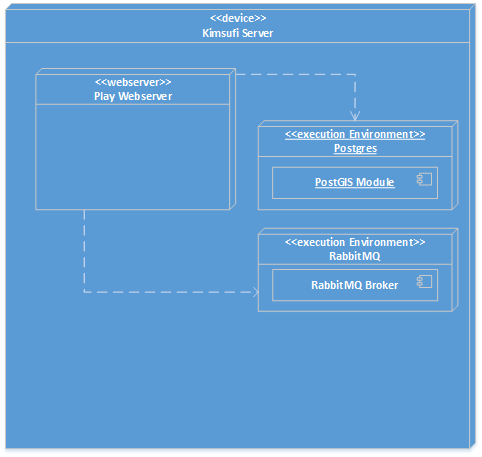
\includegraphics[width=0.75\textwidth]{images/DeploymentDiagram.png}
	\caption{Deployment Diagram}
	\label{fig:deployment-diagram}
\end{figure}


